\documentclass[11pt,a4paper]{article}
\usepackage[margin=22mm]{geometry}
\usepackage{amsmath,amssymb,bm}
\usepackage{booktabs,siunitx,graphicx,hyperref,enumitem,caption,float,array,setspace,xcolor,tabularx}
\sisetup{per-mode=symbol}
\captionsetup{font=small,labelfont=bf,skip=6pt}
\setstretch{1.08}
\setlist[itemize]{leftmargin=1.3em,itemsep=2pt,topsep=3pt}
\setlist[enumerate]{leftmargin=1.4em,itemsep=3pt,topsep=3pt}
\graphicspath{{./}}
\begin{document}

%====================================================
\begin{center}
{\LARGE\bfseries THE UNIVERSITY OF QUEENSLAND}\\[6pt]
{\large School of Mechanical and Mining Engineering}\\[14pt]
{\Large\bfseries MECH3200 -- Group Consulting Assignment B2}\\[6pt]
{\large Tower Design, Flexible-Base Dynamics and Finite-Element Model of the\\ Floating Offshore Wind Turbine}\\[8pt]
\end{center}
\vspace{5mm}
\noindent
\begin{tabular}{@{}ll@{}}
\textbf{Student Name:} & Vennkkata Reddi Cheemalapati \\
\textbf{Student Number:} & 46555991 \quad (SN$^*$ = 91) \\
% \textbf{Group members:} & James Landro (48009201), Rory Fenelon (48037615) \\   % uncomment if a group submission
\textbf{Course Code:} & MECH3200 \\
\textbf{Course Coordinator:} & Prof.\ Paul Meehan \\
\textbf{Submission Date:} & \underline{\hspace{3.5cm}} (start of Week 13) \\
\end{tabular}
\vspace{8mm}

\noindent Prof Paul Meehan\\
MECH3200 Course Coordinator\\
School of Mechanical and Mining Engineering\\
The University of Queensland\\
Queensland 4072
\vspace{5mm}

\noindent Dear Sir,
\vspace{2mm}

\noindent I, Vennkkata Reddi Cheemalapati, am the author of this assignment,
\textit{Tower Design, Flexible-Base Dynamics and Finite-Element Model of the Floating Offshore Wind Turbine (Assignment B2)}.
\vspace{2mm}

\noindent I warrant that no third-party copyrights or legal rights are infringed by this assignment.
\vspace{2mm}

\noindent All work contained in this assignment is my original work except where otherwise acknowledged.
\vspace{8mm}

\noindent Signature: \underline{\hspace{6.5cm}} \hfill Student ID: 46555991
\vspace{3mm}

\noindent Date: \underline{\hspace{4cm}}

\newpage
%====================================================
\section*{Declaration of Artificial Intelligence Use}
\addcontentsline{toc}{section}{Declaration of Artificial Intelligence Use}
In accordance with the University of Queensland's policies on the responsible use of Artificial Intelligence in assessment, the following record is provided.

\vspace{3mm}
{\renewcommand{\arraystretch}{1.3}\small
\noindent\begin{tabular}{@{}>{\raggedright\arraybackslash}p{3.1cm}p{12.8cm}@{}}
\toprule
\textbf{AI Tool Used} & Generative AI assistant (large language model) \\
\midrule
\textbf{Dates of Use} & 4 August 2026 -- 7 October 2026 \\
\midrule
\textbf{Purpose and\newline Extent} &
\begin{itemize}[leftmargin=*,nosep,itemsep=2pt]
\item Checking the Euler--Bernoulli cantilever and tip-mass frequency derivations and the modal forced-response expressions used in B2.1--B2.3.
\item Assistance writing the Python finite-element script (\texttt{fe\_model.py}, in the project repository) that implements the Timoshenko beam elements, geometric stiffness, rigid-platform constraints and modal/forced solutions used in B2.4, and the plotting scripts that produced Figures~\ref{fig:modes}--\ref{fig:frf}.
\item Identifying the inconsistency between the project-table radius of gyration and the designed tower inertia (Section~\ref{sec:b24}).
\item Report structure, LaTeX typesetting and proof-reading.
\end{itemize} \\
\midrule
\textbf{Nature of\newline Interaction} &
Technical queries on beam vibration theory, verification of intermediate numerical results for SN$^*=91$, and review of the finite-element formulation. All FE results were produced by running that script, which is published with the report (Section~\ref{sec:code}); no numerical result was accepted without checking it against the closed-form limits (Table~\ref{tab:validation}). \\
\midrule
\textbf{Sections\newline Affected} & B2.1--B2.4, figures, and this declaration. \\
\midrule
\textbf{Student\newline Contribution} &
Choice of idealisations and boundary conditions, the design decisions in B2.1--B2.3, the interpretation of the FE results and the vibration-control recommendations are my own. I have checked every analytical number in Sections~\ref{sec:b21}--\ref{sec:b23} by hand and accept full responsibility for the submitted work. \\
\bottomrule
\end{tabular}}
\vspace{6mm}

\noindent Student Number: 46555991 \hfill Date: \underline{\hspace{3.5cm}}
\vspace{4mm}

\noindent Signature: \underline{\hspace{6.5cm}}

\newpage
\tableofcontents
\newpage

%====================================================
\section{Parameters and idealisation (SN$^*$ = 91)}
%====================================================
From the project table with $L=100(1+91/200)=145.5\,\mathrm{m}$:
\begin{align*}
L_t&=1.25L=181.875\,\mathrm{m}, & M_r&=3L=436.5\,\mathrm{t}, & M_n&=1.2M_r=523.8\,\mathrm{t},\\
E&=200\,\mathrm{GPa}, & \nu&=0.25, & G&=E/[2(1+\nu)]=80\,\mathrm{GPa}, \qquad \rho=7850\,\mathrm{kg/m^3},
\end{align*}
where $E$ and $\nu$ are the AS\,4100 structural-steel values quoted in the brief. The tower is a thin-walled tube of diameter $d_t$ and wall thickness $t$, for which the table gives
\[
I=\frac{\pi d_t^3 t}{8},\qquad A=\pi d_t t,\qquad \mu=\rho A \ \ (\text{mass per unit length}).
\]
Two observations fix the design route. First, the ratio $I/A=d_t^2/8$ is independent of $t$, so every natural frequency of the bare tower depends on $d_t$ only: B2.1 (frequency) sizes the diameter and B2.2 (amplitude, which depends on $EI\propto d_t^3t$) sizes the wall. Second, the tower length and nacelle mass are fixed by the table; $d_t$ and $t$ are the outputs of this assignment, not inputs.

\paragraph{Excitation.} With the blade-tip speed limited to $V_{tip}=90.7\,\mathrm{m/s}$,
\[
\Omega_b=\frac{V_{tip}}{L}=\frac{90.7}{145.5}=0.6234\,\mathrm{rad/s},\qquad
f_{1P}=\frac{\Omega_b}{2\pi}=0.0992\,\mathrm{Hz},\qquad
f_{3P}=n_b f_{1P}=0.2976\,\mathrm{Hz}.
\]
(At the A1 design point of $30\,\mathrm{m/s}$ and $\lambda=6$ the unlimited tip speed would be $180\,\mathrm{m/s}$; the limit is reached at $U_\infty=90.7/6=15.1\,\mathrm{m/s}$, above which $\Omega_b$ is held constant by pitch control.) The design criterion is therefore
\[
f_1\ge 1.2f_{3P}=0.3572\,\mathrm{Hz}.
\]
The wind force at the rotor is $P=kU_\infty^2$ with $P(10\,\mathrm{m/s})=46.8(1+91/100)=89.39\,\mathrm{kN}$, so $k=893.9\,\mathrm{N\,s^2/m^2}$ and at the maximum wind speed $P(40)=1.430\,\mathrm{MN}$, applied at $a=0.95L_t=172.8\,\mathrm{m}$.

%====================================================
\section{B2.1 -- Tower diameter and fixed-base frequencies}\label{sec:b21}
%====================================================
\subsection*{Governing equation and characteristic equation}
Euler--Bernoulli bending of a uniform beam gives $EI\,\partial^4y/\partial x^4+\mu\,\partial^2y/\partial t^2=0$. With $y=Y(x)\cos\omega t$, $Y''''=\beta^4Y$, $\beta^4=\mu\omega^2/EI$, and
\[
Y(x)=C_1\sin\beta x+C_2\cos\beta x+C_3\sinh\beta x+C_4\cosh\beta x .
\]
The fixed--free conditions are $Y(0)=Y'(0)=0$ (built in at the platform) and $Y''(L_t)=Y'''(L_t)=0$ (zero moment and shear at the free nacelle end, nacelle inertia neglected as instructed). The first pair gives $C_4=-C_2$, $C_3=-C_1$, so
$Y=C_1(\sin\beta x-\sinh\beta x)+C_2(\cos\beta x-\cosh\beta x)$. The second pair gives the homogeneous system
\[
\begin{bmatrix}
-(\sin\beta L_t+\sinh\beta L_t) & -(\cos\beta L_t+\cosh\beta L_t)\\
-(\cos\beta L_t+\cosh\beta L_t) & \ \ \sin\beta L_t-\sinh\beta L_t
\end{bmatrix}\!\begin{bmatrix}C_1\\C_2\end{bmatrix}=\mathbf 0,
\]
whose determinant, after using $\sin^2+\cos^2=1$ and $\cosh^2-\sinh^2=1$, reduces to the cantilever characteristic equation
\begin{equation}
1+\cos(\beta L_t)\cosh(\beta L_t)=0 \quad\Rightarrow\quad \beta_nL_t=1.8751,\ 4.6941,\ 7.8548,\ \ldots
\label{eq:cant}
\end{equation}
Hence
\begin{equation}
f_n=\frac{\omega_n}{2\pi}=\frac{(\beta_nL_t)^2}{2\pi L_t^2}\sqrt{\frac{EI}{\mu}}
=\frac{(\beta_nL_t)^2}{2\pi L_t^2}\sqrt{\frac{E}{\rho}}\;\frac{d_t}{\sqrt 8},
\label{eq:fn}
\end{equation}
using $EI/\mu=E d_t^2/(8\rho)$ for the thin tube. The mode shapes are
\begin{equation}
Y_n(x)=\cosh\beta_nx-\cos\beta_nx-\sigma_n(\sinh\beta_nx-\sin\beta_nx),\qquad
\sigma_n=\frac{\sinh\beta_nL_t-\sin\beta_nL_t}{\cosh\beta_nL_t+\cos\beta_nL_t}.
\label{eq:shape}
\end{equation}

\subsection*{Diameter}
Setting $f_1=1.2f_{3P}$ in Eq.~\eqref{eq:fn} and solving for $d_t$:
\[
d_t=\frac{2\pi L_t^2\sqrt{8}\,f_{req}}{(1.8751)^2\sqrt{E/\rho}}
=\frac{2\pi(181.875)^2\sqrt 8\,(0.3572)}{3.5160\times 5047.0}
=\mathbf{11.83\,\mathrm{m}} .
\]
\begin{table}[H]
\centering
\caption{Fixed-base natural frequencies of the bare tower, $d_t=11.83\,\mathrm{m}$ (any wall thickness).}
\begin{tabular}{@{}cccc@{}}
\toprule
Mode & $\beta_nL_t$ & $f_n$ (Hz) & Ratio to $f_{3P}$ \\
\midrule
1 & 1.8751 & \textbf{0.357} & 1.20 \\
2 & 4.6941 & 2.238 & 7.52 \\
3 & 7.8548 & 6.267 & 21.1 \\
\bottomrule
\end{tabular}
\end{table}
Mode~1 is single-curvature with the nacelle at the antinode; mode~2 has one interior node at $x\approx0.78L_t$ and mode~3 two nodes at $0.50L_t$ and $0.87L_t$ (Figure~\ref{fig:anmodes}, solid lines). Only mode~1 is close to the blade-passing band; modes~2 and~3 sit an order of magnitude higher.

%====================================================
\section{B2.2 -- Wall thickness from the tip-amplitude limit}\label{sec:b22}
%====================================================
\subsection*{Modal forced response}
Expanding $y(x,t)=\sum_n Y_n(x)q_n(t)$ with $Y_n$ normalised to unity at the tip, orthogonality of the cantilever modes decouples the equations of motion into
\[
m_n\ddot q_n+m_n\omega_n^2q_n=P\,Y_n(a)\sin\Omega t,\qquad
m_n=\mu\!\int_0^{L_t}\!Y_n^2\,dx=0.250\,\mu L_t \ (\text{for all three modes}).
\]
The steady-state tip amplitude under a point force of amplitude $P$ at $x=a$ and frequency $\Omega$ is therefore
\begin{equation}
X_{tip}(\Omega)=\sum_n\frac{P\,Y_n(a)}{m_n\omega_n^2}\,\frac{1}{\sqrt{(1-r_n^2)^2+(2\zeta r_n)^2}},\qquad r_n=\frac{\Omega}{\omega_n},
\label{eq:forced}
\end{equation}
with $Y_1(a)=0.931$, $Y_2(a)=0.761$, $Y_3(a)=0.608$ at $a=0.95L_t$. The force acts at both $f_{1P}$ and $f_{3P}$ with the same amplitude $P$; the worst case is the in-phase sum of the two components. The design is made with $\zeta=0$ (conservative); the $1\%$ damping used in B2.4 changes the result by only $0.1\%$ because $r_1=0.833$ is not close to unity.

\subsection*{Thickness}
Since $m_n\omega_n^2=0.25\mu L_t\omega_n^2\propto t$ (frequencies fixed by $d_t$, mass $\propto t$), $X_{tip}\propto1/t$. Requiring $X_{tip}\le0.007L_t=1.273\,\mathrm{m}$:
\begin{align*}
\text{at }f_{3P}:\ r_1&=0.833,\ \ \frac{1}{1-r_1^2}=3.27; &
\text{at }f_{1P}:\ r_1&=0.278,\ \ \frac{1}{1-r_1^2}=1.08,\\
X_{3P}&=\frac{0.953}{t/0.0689}\,\mathrm{m}, & X_{1P}&=\frac{0.320}{t/0.0689}\,\mathrm{m},
\end{align*}
\[
X_{1P}+X_{3P}=1.273\,\mathrm{m}\quad\Rightarrow\quad \mathbf{t=68.9\,\mathrm{mm}}\ \ (d_t/t=172).
\]
Check: $I=\pi d_t^3t/8=44.8\,\mathrm{m^4}$; the static tip deflection under $P$ at $a$ is $\delta=Pa^2(3L_t-a)/(6EI)=0.296\,\mathrm{m}$, and $\delta\times3.27\,(\text{DAF at }3P)=0.97\,\mathrm{m}$ agrees with the first-mode term $0.953\,\mathrm{m}$. Modes~2 and~3 contribute $<2\%$. The tower mass is $\mu L_t=3658\,\mathrm{t}$.

%====================================================
\section{B2.3 -- Effect of the nacelle mass and design action}\label{sec:b23}
%====================================================
\subsection*{Rayleigh (equivalent-mass) prediction}
With the static cantilever deflection shape $\psi(x)=(3L_tx^2-x^3)/(2L_t^3)$ as the trial function, Rayleigh's quotient gives an equivalent tip stiffness $k_e=3EI/L_t^3$ and an equivalent tip mass $\int_0^{L_t}\mu\psi^2dx=\tfrac{33}{140}\mu L_t$. Adding the nacelle $M_n$ at the tip,
\begin{equation}
\frac{f_1'}{f_1}=\sqrt{\frac{\tfrac{33}{140}\mu L_t}{M_n+\tfrac{33}{140}\mu L_t}}
=\sqrt{\frac{0.2357}{0.1432+0.2357}}=0.789\quad\Rightarrow\quad \Delta f_1=-21.1\%,
\label{eq:rayleigh}
\end{equation}
with $\alpha=M_n/\mu L_t=523.8/3658=0.1432$.

\subsection*{Exact solution and error estimate}
Keeping the exact mode shape, the free-end shear condition becomes $EIY'''(L_t)=-M_n\omega^2Y(L_t)$ (inertia force of the tip mass) while $Y''(L_t)=0$. Substituting the general solution and eliminating the constants as in Section~\ref{sec:b21} gives the tip-mass characteristic equation
\begin{equation}
1+\cos\beta L_t\cosh\beta L_t-\alpha\,\beta L_t\,(\sin\beta L_t\cosh\beta L_t-\cos\beta L_t\sinh\beta L_t)=0,
\label{eq:tipmass}
\end{equation}
which reduces to Eq.~\eqref{eq:cant} for $\alpha=0$. Solving numerically for $\alpha=0.1432$: $\beta_1L_t=1.6727$, so
\[
\frac{f_1'}{f_1}=\Bigl(\frac{1.6727}{1.8751}\Bigr)^2=0.796\quad\Rightarrow\quad \Delta f_1=-20.4\%,\qquad f_1'=0.284\,\mathrm{Hz}.
\]
The Rayleigh estimate ($-21.1\%$) is in error by $0.9\%$ of the frequency, i.e.\ it slightly over-predicts the drop. The direction is as expected: Rayleigh's quotient with the massless static shape gives an upper bound on $f_1$ (3.567 vs the exact 3.516 in Eq.~\eqref{eq:fn}) and the same shape under-estimates the tip-mass participation, so the ratio is slightly low. The higher modes drop less because their tip amplitude is a smaller fraction of the modal mass: $f_2'=1.906\,\mathrm{Hz}$ ($-14.8\%$), $f_3'=5.532\,\mathrm{Hz}$ ($-11.7\%$).

\subsection*{Consequence for the B2.1--B2.2 design}
$f_1'=0.284\,\mathrm{Hz}$ is only $0.955f_{3P}$: the nacelle mass alone moves the designed tower from $20\%$ above blade passing to \emph{within 5\% of 3P resonance}. The B2.1 criterion is violated and the B2.2 amplitude would grow without bound at $r\to1$. The wall thickness cannot fix this ($f_1$ is independent of $t$ for the bare tower, and increasing $t$ only lowers $\alpha$ weakly), so the diameter must increase.

\paragraph{Action.} Hold $t=68.9\,\mathrm{mm}$ and increase $d_t$ until Eq.~\eqref{eq:tipmass} returns $f_1'=0.357\,\mathrm{Hz}$ (the mass ratio changes with $d_t$, so this is solved iteratively):
\[
\boxed{d_t=14.37\,\mathrm{m}\ (+21.5\%),\qquad t=68.9\,\mathrm{mm},\qquad d_t/t=209,}\qquad
\alpha=0.118,\ \ \mu L_t=4444\,\mathrm{t}.
\]
\begin{table}[H]
\centering
\caption{Redesigned tower, fixed base, with nacelle mass (Euler--Bernoulli).}
\begin{tabular}{@{}ccccc@{}}
\toprule
Mode & $\beta_nL_t$ & $f_n$ (Hz) & Ratio to $f_{3P}$ & Tip amplitude at $P(40)$ \\
\midrule
1 & 1.7012 & \textbf{0.357} & 1.20 & $X_{1P}+X_{3P}=0.18+0.54=0.72\,\mathrm{m}$ \\
2 & 4.3689 & 2.356 & 7.9 & $<0.01$ m \\
3 & 7.4181 & 6.791 & 22.8 & -- \\
\bottomrule
\end{tabular}
\end{table}
The tip amplitude is $0.72\,\mathrm{m}$, $56\%$ of the allowable $1.273\,\mathrm{m}$, because $EI$ grew by $(14.37/11.83)^3=1.79$. A thinner wall would also satisfy both criteria mathematically, but an unconstrained joint solution drifts to $d_t\approx18\,\mathrm{m}$, $t\approx19\,\mathrm{mm}$ ($d_t/t\approx940$), which is unacceptable for local shell buckling; $d_t/t\approx200$ is retained. Sensitivity: if the rotor mass $M_r$ is also lumped at the tip ($\alpha=0.216$), $f_1'$ falls to $0.317\,\mathrm{Hz}$ and a further $\approx13\%$ diameter increase would be needed.

\begin{figure}[H]
\centering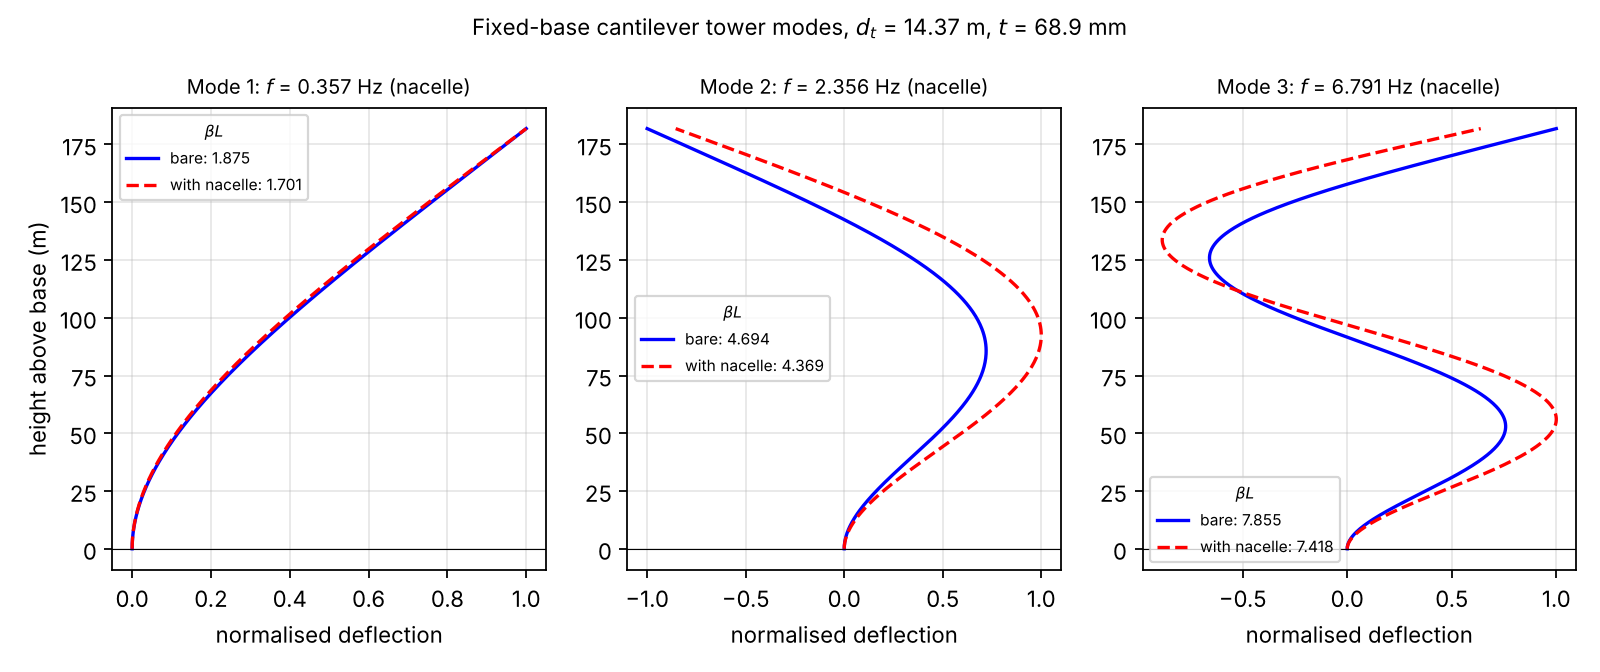
\includegraphics[width=0.95\textwidth]{tower_modes_analytical.png}
\caption{Fixed-base mode shapes of the redesigned tower from Eq.~\eqref{eq:shape} without (solid) and with (dashed) the nacelle tip mass. The tip mass pulls the node of mode~2 toward the base and increases the tip slope of mode~1.}
\label{fig:anmodes}
\end{figure}

\subsection*{Reassessment of the boundary condition}
The fixed root is the weak assumption. In A2 the platform pitch and roll modes were found at $0.216$ and $0.227\,\mathrm{Hz}$ with surge/sway at $0.049\,\mathrm{Hz}$ -- the same decade as the tower fundamental. A rotational spring at the base always lowers the tower frequency, and the platform's rigid pitch inertia will couple with tower bending. The fixed-base $f_1=0.357\,\mathrm{Hz}$ is therefore an upper bound; the real fundamental is a coupled pitch--bending mode that is quantified in Section~\ref{sec:b24}.

%====================================================
\section{B2.4 -- Finite-element model of the floating system}\label{sec:b24}
%====================================================
\subsection*{Model}
The designed configuration is shown in Figures~\ref{fig:geom}--\ref{fig:geom2}. A planar (surge $X$, heave $Y$, pitch $\theta$) finite-element model of it was built in Python (\texttt{fe\_model.py}; source and results in the repository, Section~\ref{sec:code}):
\begin{itemize}
\item \textbf{Tower}: 40 two-node Timoshenko beam elements (Przemieniecki stiffness with shear parameter $\phi=12EI/(k_sGAL_e^2)$, consistent mass with rotary inertia, $k_s=0.5$ for a thin circular tube), $d_t=14.37\,\mathrm{m}$, $t=68.9\,\mathrm{mm}$. Nacelle $M_n$ as a point mass at the tip.
\item \textbf{Platform}: rigid body with DOF $(X,Y,\theta)$ at its centre of mass. The tower base node is $10\,\mathrm{m}$ above the COM and is tied by the rigid-body constraint $v_{base}=X-10\theta$, $\theta_{base}=\theta$ (master--slave transformation). The four A2 mounts at $(\pm b,-a)=(\pm40,-7)\,\mathrm{m}$ give the A2.1 stiffness matrix (surge, heave, pitch)
\[
\mathbf K_p=\begin{bmatrix}4k_x&0&4k_xa\\0&4k_y&0\\4k_xa&0&4k_xa^2+4k_yb^2\end{bmatrix},\qquad k_x=0.5\,\mathrm{MN/m},\quad k_y=\rho_{sw}gA_{ky}=10.06\,\mathrm{MN/m}.
\]
\item \textbf{Power cable}: 40 tensioned beam elements ($E_{pc}=10\,\mathrm{GPa}$, $d_{pc}=0.24\,\mathrm{m}$, $\rho_{pc}=3000\,\mathrm{kg/m^3}$, $L_{pc}=160.05\,\mathrm{m}$) with the geometric stiffness $T\mathbf K_g$ for $T_{pc}=400\,\mathrm{kN}$, hanging from the platform COM: top translation tied to $X$, rotation free (pin); bottom pinned to the seabed.
\item \textbf{Damping}: $1\%$ modal, used in the forced response.
\end{itemize}
\begin{figure}[H]
\centering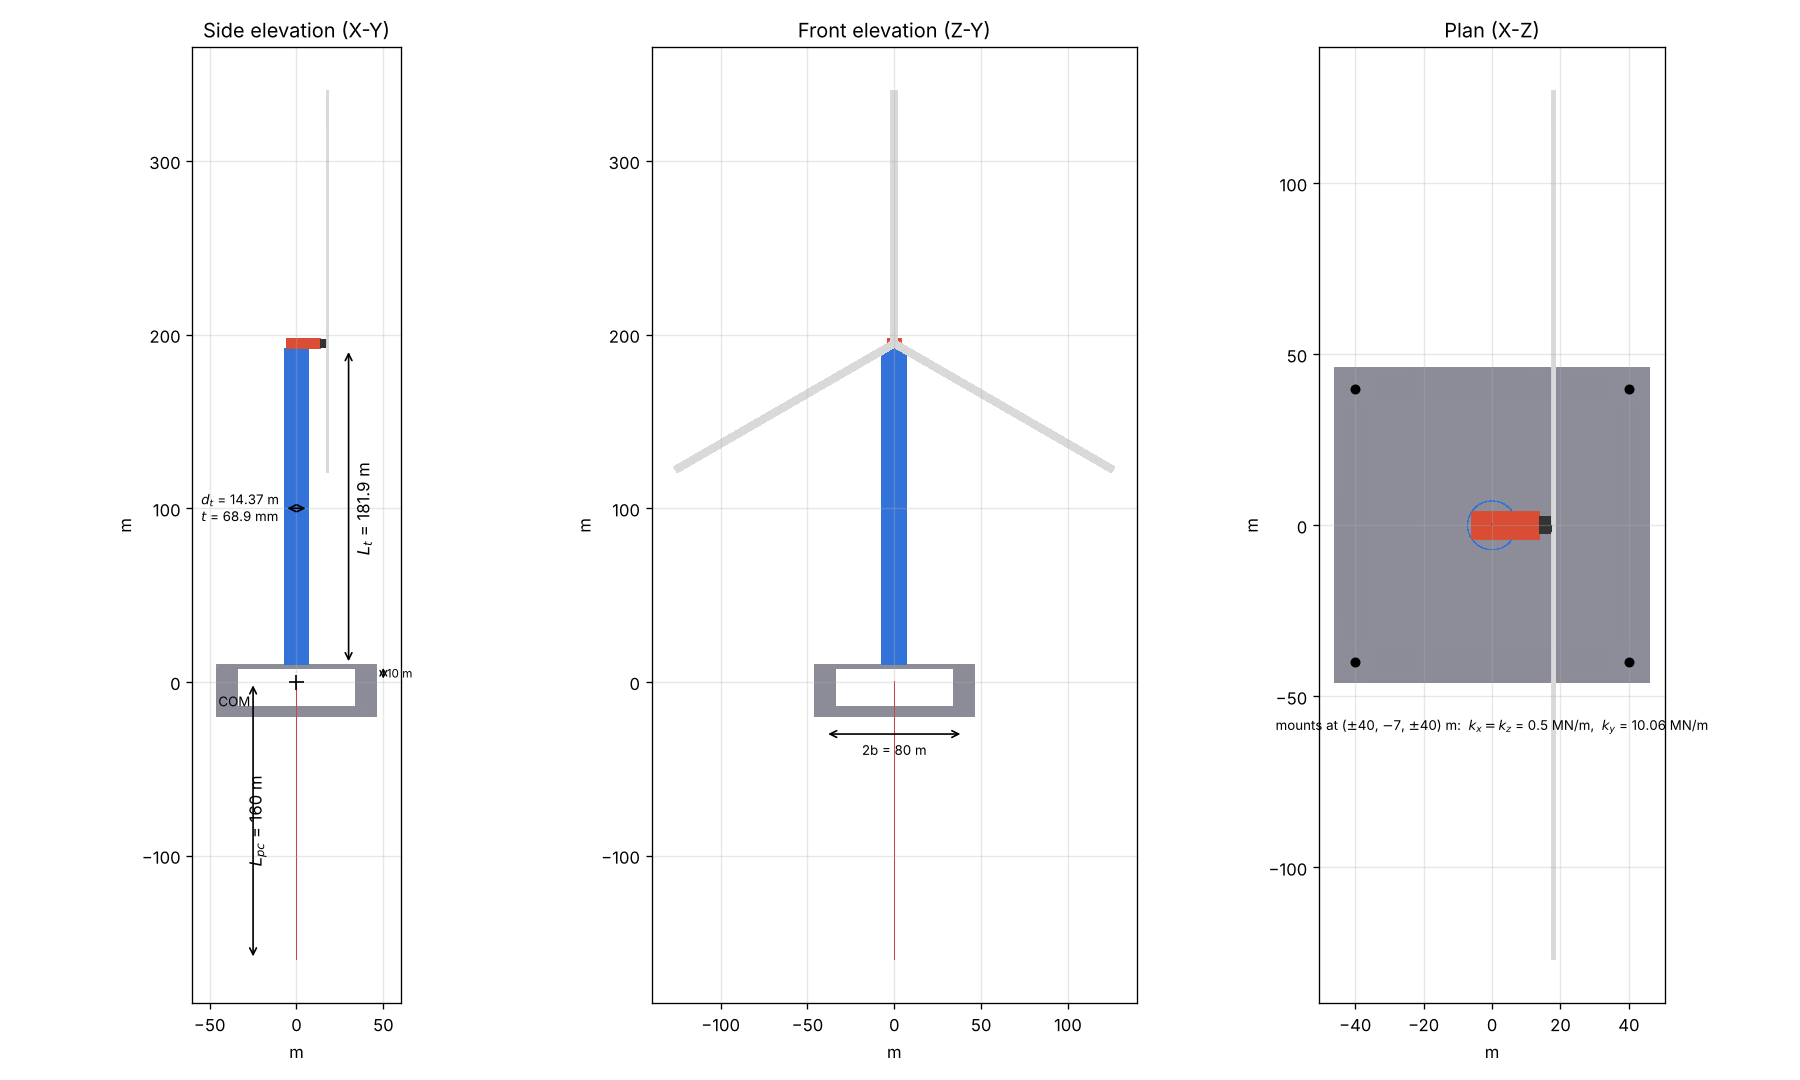
\includegraphics[width=\textwidth]{step_3view.png}
\caption{Geometry of the designed configuration (STEP file \texttt{MECH3200\_B2\_46555991.step} supplied, generated by \texttt{make\_step.py}). Mount pads mark the four A2 isolator positions at $(\pm b,-a,\pm b)$; the cable is pinned at the platform centre of mass and at the seabed. The FE model of this section idealises this geometry as beam elements, a rigid platform and point masses.}
\label{fig:geom}
\end{figure}
\begin{figure}[H]
\centering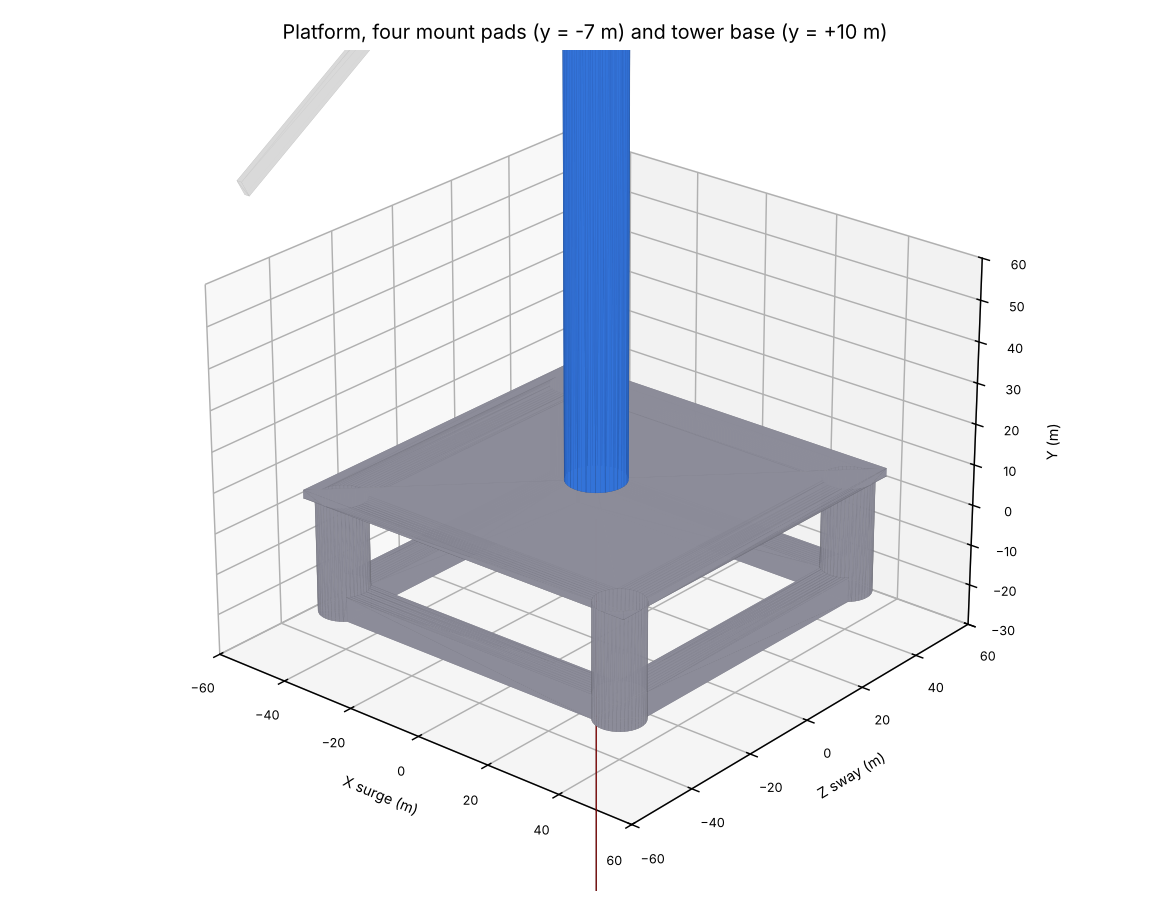
\includegraphics[width=0.48\textwidth]{step_platform.png}\hfill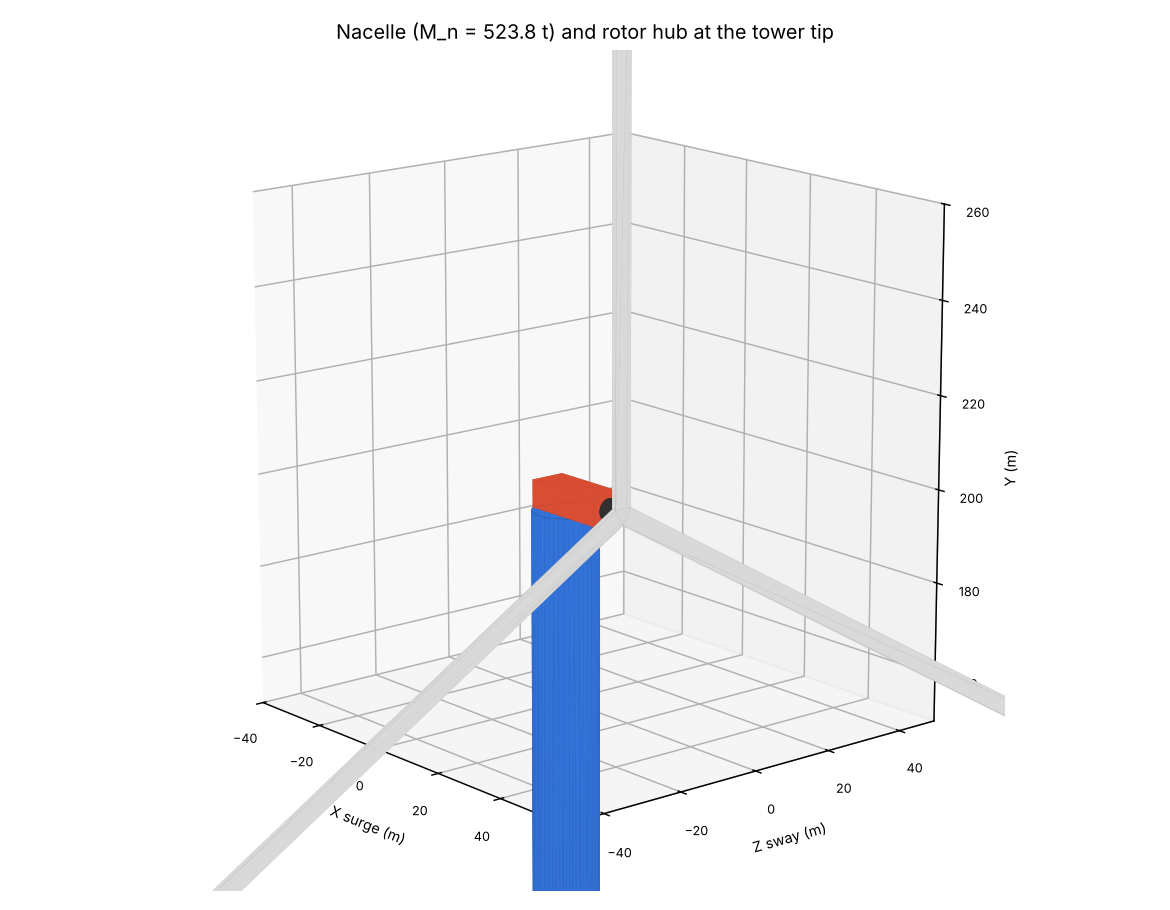
\includegraphics[width=0.48\textwidth]{step_nacelle.png}
\caption{Platform with the tower base at $y=+10\,\mathrm{m}$ above the centre of mass (left) and the nacelle at the tower tip (right), rendered from the STEP geometry.}
\label{fig:geom2}
\end{figure}
\paragraph{Mass bookkeeping.} The table gives a \emph{total} rigid-body mass $M=20\,853\,\mathrm{t}$ and radius of gyration $k_{xy}=41\,\mathrm{m}$. The FE model represents the tower ($4444\,\mathrm{t}$) and nacelle explicitly, so the lumped platform mass is $M_p=M-\mu L_t-M_n=15\,885\,\mathrm{t}$ (heave uses the full $M$, the tower being axially rigid). The rotational inertia cannot be split the same way: the tower and nacelle alone contribute $7.7\times10^{10}\,\mathrm{kg\,m^2}$ about the COM, more than twice the table's total $Mk_{xy}^2=3.5\times10^{10}$. The table's rigid-body data are therefore inconsistent with a $182\,\mathrm{m}$ tower of this mass; the table value is assigned to the platform hull and the tower/nacelle inertia is added by the elements. This is flagged to the client: the A2 pitch frequency was computed with an inertia that cannot contain the tower.

\subsection*{Validation against the closed-form results}
\begin{table}[H]
\centering
\caption{FE limiting cases versus the analytical solutions of A2, B1 and B2.1--B2.3.}
\label{tab:validation}
\begin{tabular}{@{}llcc@{}}
\toprule
Case (FE switches) & Quantity & Analytical & FE \\
\midrule
Fixed base, EB, no nacelle, $d_t=11.83$ m & $f_1$ & 0.3572 & 0.3572 \\
Fixed base, EB, nacelle, $d_t=11.83$ m & $f_1$ & 0.2842 & 0.2842 \\
Fixed base, EB, nacelle, $d_t=14.37$ m & $f_1,f_2,f_3$ & 0.357, 2.356, 6.791 & 0.357, 2.356, 6.791 \\
Cable pinned--pinned, tensioned (B1.3) & $f_{tb,1\ldots8}$ & 0.170 \ldots 1.423 & 0.170 \ldots 1.423 (all 8 to 4 s.f.) \\
Cable, $T=0$ (B1.2) & $f_{b,1\ldots3}$ & 0.0067, 0.0269, 0.0605 & 0.0067, 0.0269, 0.0605 \\
Platform only, surge / heave (A2.1) & $f$ & 0.0492 / 0.2210 & 0.0490 / 0.2210 \\
\bottomrule
\end{tabular}
\end{table}
The exact agreement of the eight tensioned-cable modes confirms numerically the B1.3 result that $\omega_{tb}^2=\omega_s^2+\omega_b^2$ is exact for pinned ends.

\subsection*{Timoshenko versus Euler--Bernoulli}
On the fixed-base tower with nacelle, shear deformation and rotary inertia lower the frequencies to $f_1=0.354$ ($-0.9\%$), $f_2=2.216$ ($-5.9\%$), $f_3=5.919\,\mathrm{Hz}$ ($-12.8\%$). The fundamental is barely affected because $L_t/d_t=12.7$ and the first mode is long-wavelength; the correction grows with mode number as the half-wavelength approaches the diameter. For B2.1 the Euler--Bernoulli design is adequate; the $0.9\%$ reduction leaves $f_1/f_{3P}=1.19$, marginally under the $1.2$ target, and is absorbed by the margin in the flexible-base redesign below.

\subsection*{Flexible-base results}
\begin{table}[H]
\centering
\caption{Undamped natural frequencies of the complete flexible-base model (Timoshenko elements, cable tension on) compared with the analytical values. Planar model: sway, roll and yaw are out of plane (sway $=$ surge by symmetry; yaw $=0.070\,\mathrm{Hz}$ after correcting the A2 yaw stiffness to $4(k_x+k_z)b^2$).}
\label{tab:fe}
\small
\begin{tabular}{@{}cp{5.2cm}p{2.5cm}p{2.6cm}p{2.9cm}@{}}
\toprule
FE mode & Character & FE $f$ (Hz) & Analytical (Hz) & Source / comment \\
\midrule
1 & Surge (cable moves with platform) & 0.0490 & 0.0492 & A2.1 \\
2 & \textbf{Coupled pitch + tower bending (in phase)} & \textbf{0.136} & 0.357 fixed base; 0.216 rigid pitch & B2.1--3, A2.1 \\
3 & Cable mode 1 & 0.170 & 0.170 & B1.3, below VIV band \\
4 & Heave & 0.221 & 0.221 & A2.1 \\
5 & Cable mode 2 & 0.340 & 0.340 & B1.3 \\
6 & Cable mode 3 & 0.512 & 0.512 & B1.3 \\
7 & Coupled pitch + bending (anti-phase) & 0.603 & -- & new mode \\
8--11 & Cable modes 4--7 & 0.687, 0.864, 1.046, 1.232 & 0.687, 0.864, 1.046, 1.232 & B1.3 \\
\bottomrule
\end{tabular}
\end{table}
\begin{figure}[H]
\centering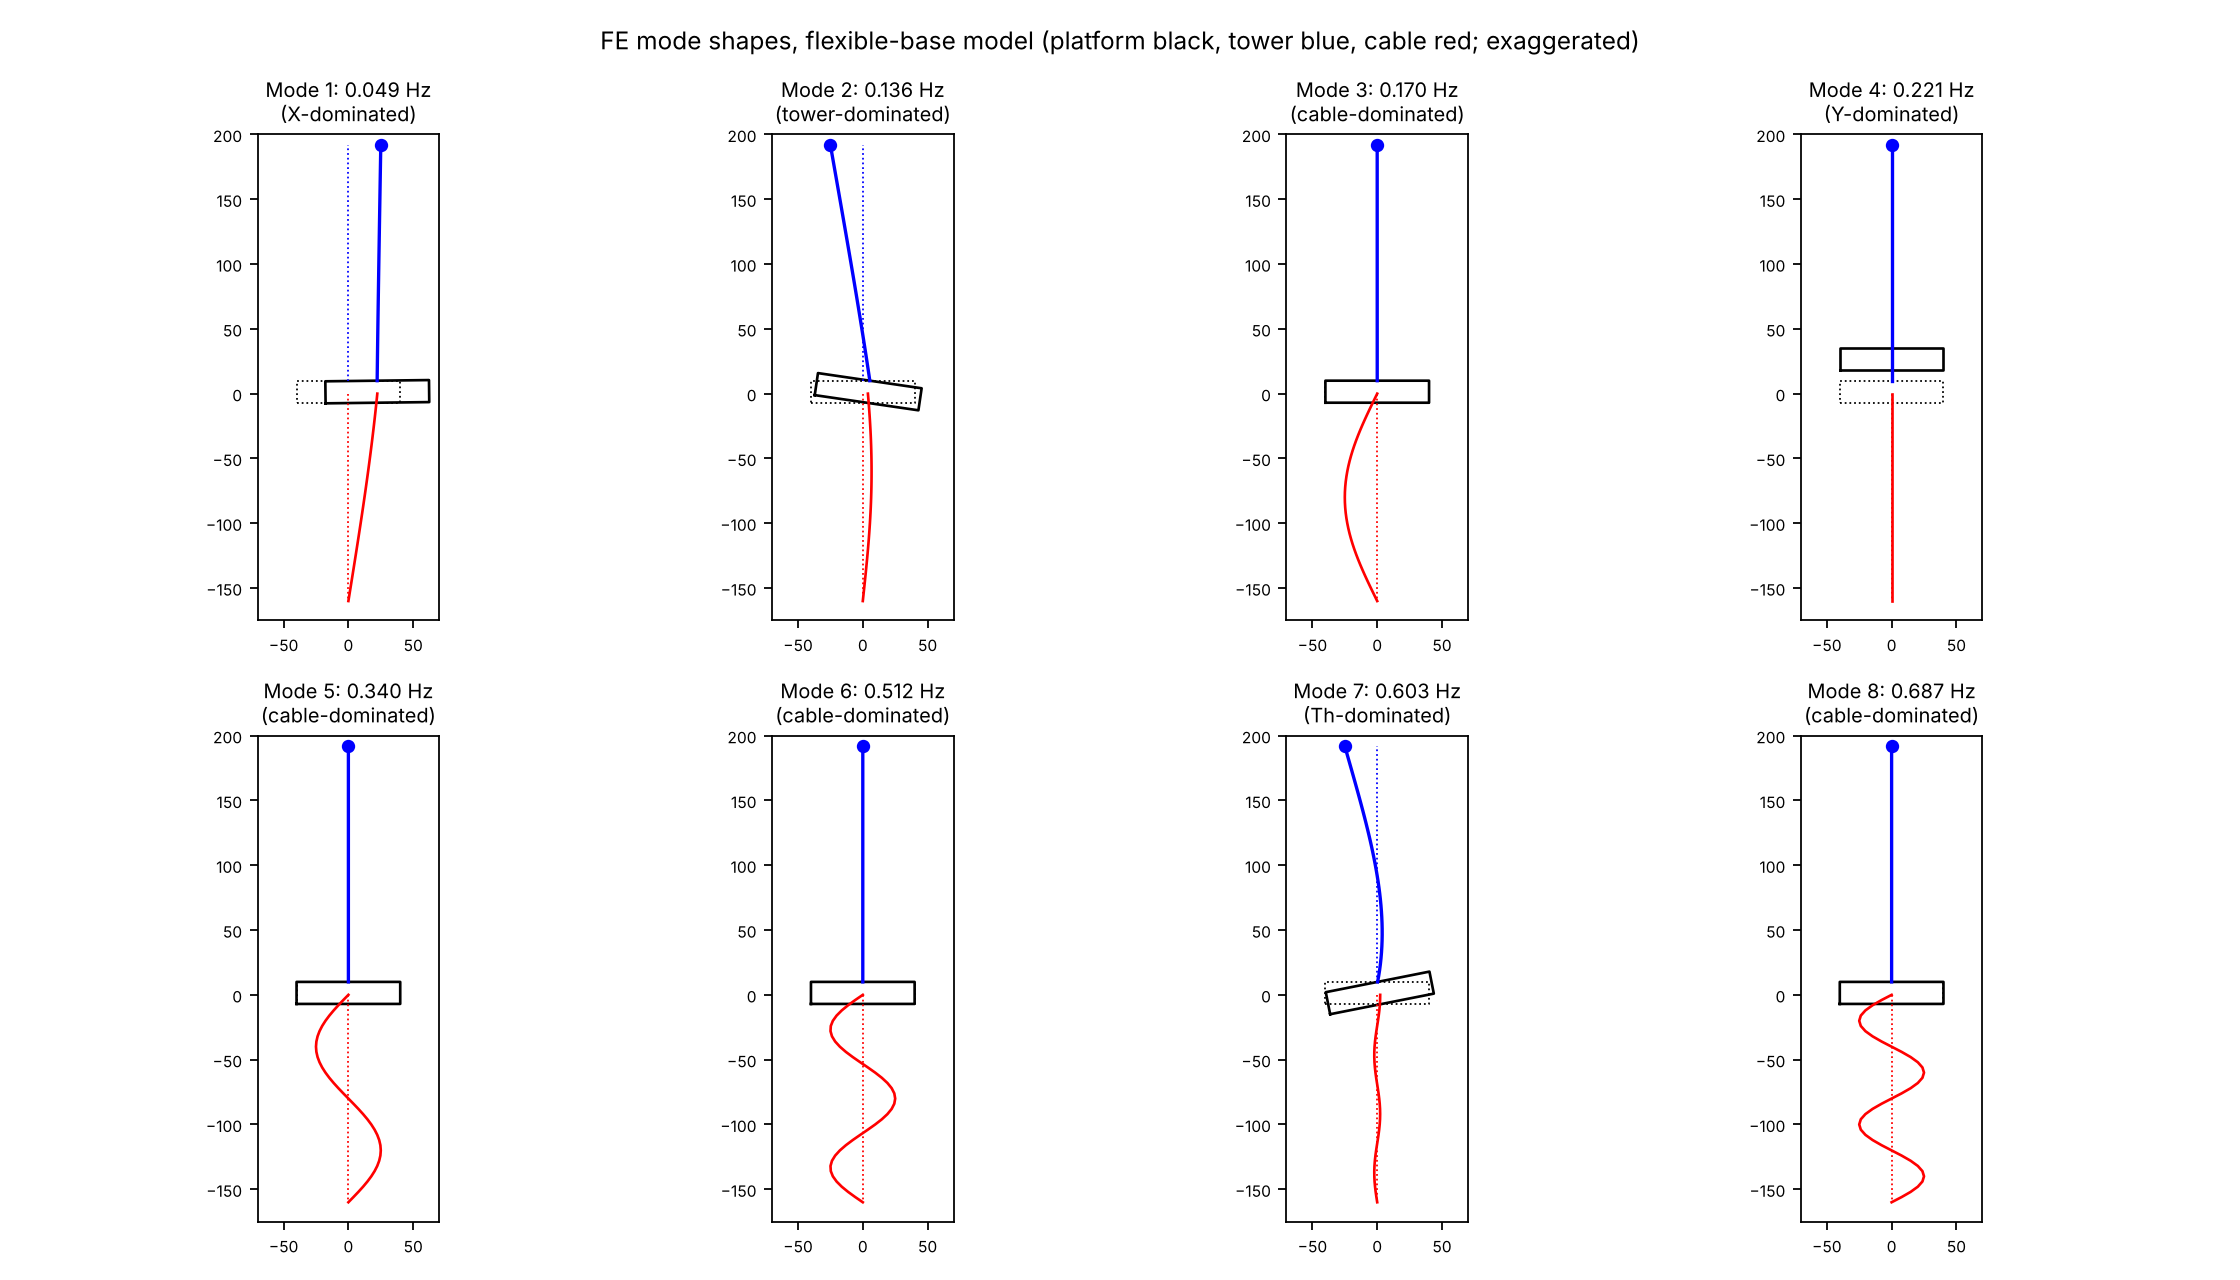
\includegraphics[width=\textwidth]{fe_modes.png}
\caption{First eight FE mode shapes (platform black, tower blue, cable red; displacements exaggerated).}
\label{fig:modes}
\end{figure}

\paragraph{Discussion.}
\begin{enumerate}
\item \textbf{Fixed root versus flexible base.} Releasing the root replaces the $0.357\,\mathrm{Hz}$ cantilever mode by a pair of coupled modes. Rigid pitch of the platform with the explicit tower inertia would be $f_\theta=\frac1{2\pi}\sqrt{(4k_xa^2+4k_yb^2)/(J_p+J_{tower})}=0.121\,\mathrm{Hz}$; coupling with bending gives $0.136\,\mathrm{Hz}$ (platform pitches and the tower bends the same way, Figure~\ref{fig:tower1}) and $0.603\,\mathrm{Hz}$ (anti-phase). The fundamental is $62\%$ below the fixed-base value: the fixed-root assumption of B2.1 is not conservative for resonance placement.
\item \textbf{Resonance check.} At the tip-speed limit, $f_{1P}=0.099$ and $f_{3P}=0.298\,\mathrm{Hz}$. The coupled mode at $0.136\,\mathrm{Hz}$ is $37\%$ above 1P but 3P sweeps through it at $\Omega_b=2\pi(0.136)/3=0.285\,\mathrm{rad/s}$, i.e.\ $V_{tip}=41.4\,\mathrm{m/s}$, $U_\infty=6.9\,\mathrm{m/s}$ at $\lambda=6$ -- inside the $5$--$40\,\mathrm{m/s}$ operating range. The force there is small ($P=42.6\,\mathrm{kN}$), but with $1\%$ damping the FE peak response (Figure~\ref{fig:frf}) is $0.82\,\mathrm{m}$ absolute and $1.88\,\mathrm{m}$ relative to the pitched platform -- the latter already exceeds the $0.7\%L_t$ limit at a wind speed of only $6.9\,\mathrm{m/s}$. The $12\,\mathrm{s}$ wave ($0.083\,\mathrm{Hz}$) sits between surge ($0.049$) and the coupled mode ($0.136$) with $r=0.61$: platform pitch from waves is amplified into the tower rather than isolated.
\item \textbf{Repeat of B2.2 (tip amplitude at $P(40)$, $1\%$ damping).} Fixed base: $X_{1P}+X_{3P}=0.18+0.57=0.75\,\mathrm{m}$ (agrees with the $0.72\,\mathrm{m}$ of Section~\ref{sec:b23}; the difference is Timoshenko plus nodal load lumping). Flexible base: absolute tip motion $0.93+0.14=1.06\,\mathrm{m}$ (passes), but the \emph{elastic} tip deflection relative to the pitched platform -- the quantity that governs blade--tower clearance -- is $2.63+0.35=2.98\,\mathrm{m}$, $2.3\times$ the $0.7\%L_t$ limit, because 1P now lies at $r=0.73$ on the $0.136\,\mathrm{Hz}$ mode. The B2.2 wall thickness, sized on a fixed root, is insufficient once the base is flexible.
\item \textbf{Repeat of A2.1 / A2.3 / A2.4.} Surge ($0.049\,\mathrm{Hz}$) and heave ($0.221\,\mathrm{Hz}$) are reproduced by the FE model. The dominant mode for the $12\,\mathrm{s}$ wave is not in the planar model: it is the yaw (twisting) mode, whose stiffness from potential energy is $k_{T}=4(k_xb_{yz}^2+k_zb_{xy}^2)=6.4\times10^9\,\mathrm{N\,m/rad}$ and inertia $M\rho_{xz}^2=3.34\times10^{10}\,\mathrm{kg\,m^2}$, giving $f_{yaw}=0.0697\,\mathrm{Hz}$ -- only $16\%$ below the $0.083\,\mathrm{Hz}$ wave, so $r=1.196$ and $T=2.28$ (the A2 submission used half this stiffness, $0.049\,\mathrm{Hz}$, and is corrected here). For an eight-fold reduction of the worst-case transmissibility the mooring stiffness, and hence pretension, must fall by $68.6\%$: $f_{yaw}\to0.039\,\mathrm{Hz}$, $r=2.13$, $T=0.286$. Re-running the FE with $k_x=0.314k_x$ gives surge $0.0275\,\mathrm{Hz}$ ($r=3.03$, $T=0.126$) while the coupled pitch--bending mode is untouched ($0.1355\,\mathrm{Hz}$) because it is governed by $4k_yb^2$, not $k_x$. The equivalent A2.4 geometric change follows from the inclined-cable stiffness. A straight cable of length $L$ under pretension $T$ (axial stiffness neglected) has transverse geometric stiffness $T/L$; a horizontal platform displacement $x$ has a component $x\sin\theta$ perpendicular to a cable inclined at $\theta$ to the horizontal, producing a transverse restoring force $(T/L)x\sin\theta$ whose horizontal component is $(T/L)x\sin^2\theta$, so $k_x=(T/L)\sin^2\theta$. With the anchor depth fixed, $L=D/\sin\theta$ and $k_x=(T/D)\sin^3\theta$. At constant pretension the required stiffness ratio therefore gives $\sin^3\theta_{new}/\sin^3 40^\circ=1-0.686\Rightarrow\theta_{new}=25.9^\circ$ (the cable must be laid flatter, lengthening it by $\sin40^\circ/\sin25.9^\circ=1.47$).
\item \textbf{Repeat of B1.3--B1.4.} The cable modes are unchanged by the moving platform (participation of $X$ in cable modes $<0.1\%$); modes 2--7 ($0.340$--$1.232\,\mathrm{Hz}$) remain inside the $0.25$--$1.25\,\mathrm{Hz}$ VIV band, and removing the tension collapses them to the B1.2 bending values, confirming the cable is tension-dominated. No cable mode coincides with a platform or tower mode (nearest: cable mode~1 at $0.170$ vs coupled mode $0.136$, $25\%$ apart), so B1.4's conclusion stands: doubling the cable damping halves every locked-in amplitude, whereas retuning tension or diameter cannot clear the band.
\item \textbf{Shear and tension.} Switching Timoshenko off changes the coupled modes by $<1\%$ ($0.1361\to0.1363$, $0.603\to0.608\,\mathrm{Hz}$); cable tension is essential (without it the cable modes fall by a factor of $\approx25$ and would crowd the wave band).
\end{enumerate}
\begin{figure}[H]
\centering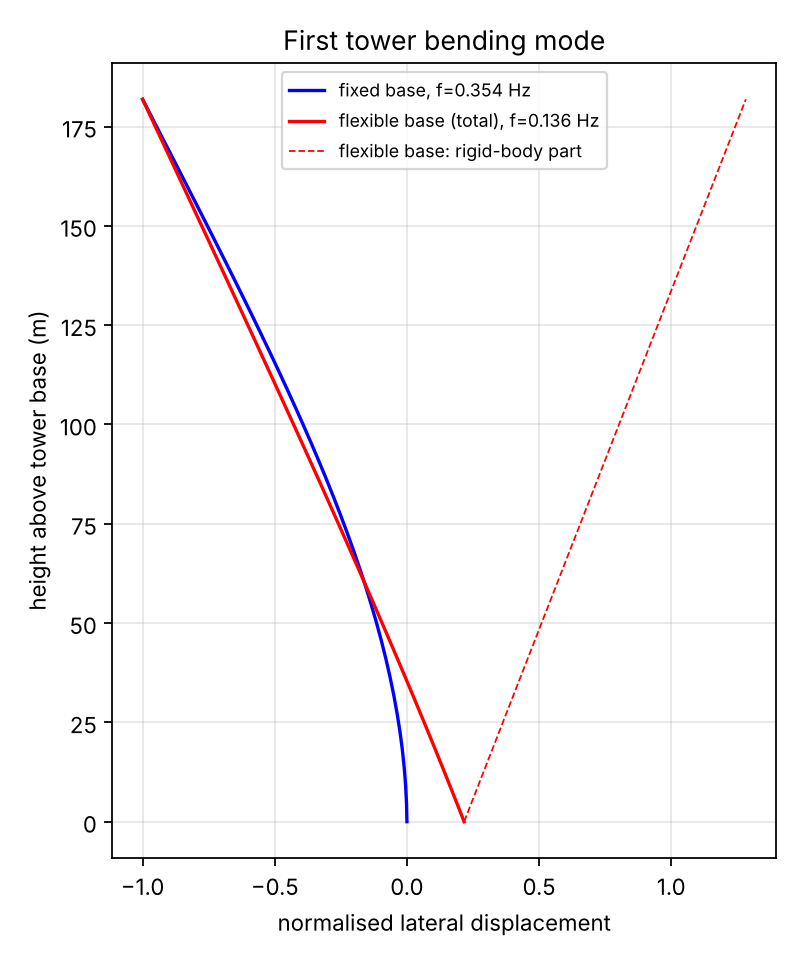
\includegraphics[width=0.55\textwidth]{fe_tower_mode1.png}
\caption{First tower bending mode: fixed base (blue) versus the coupled flexible-base mode (red). The dashed line is the rigid-body (pitch) part of the flexible-base mode; the elastic deflection is the difference.}
\label{fig:tower1}
\end{figure}
\begin{figure}[H]
\centering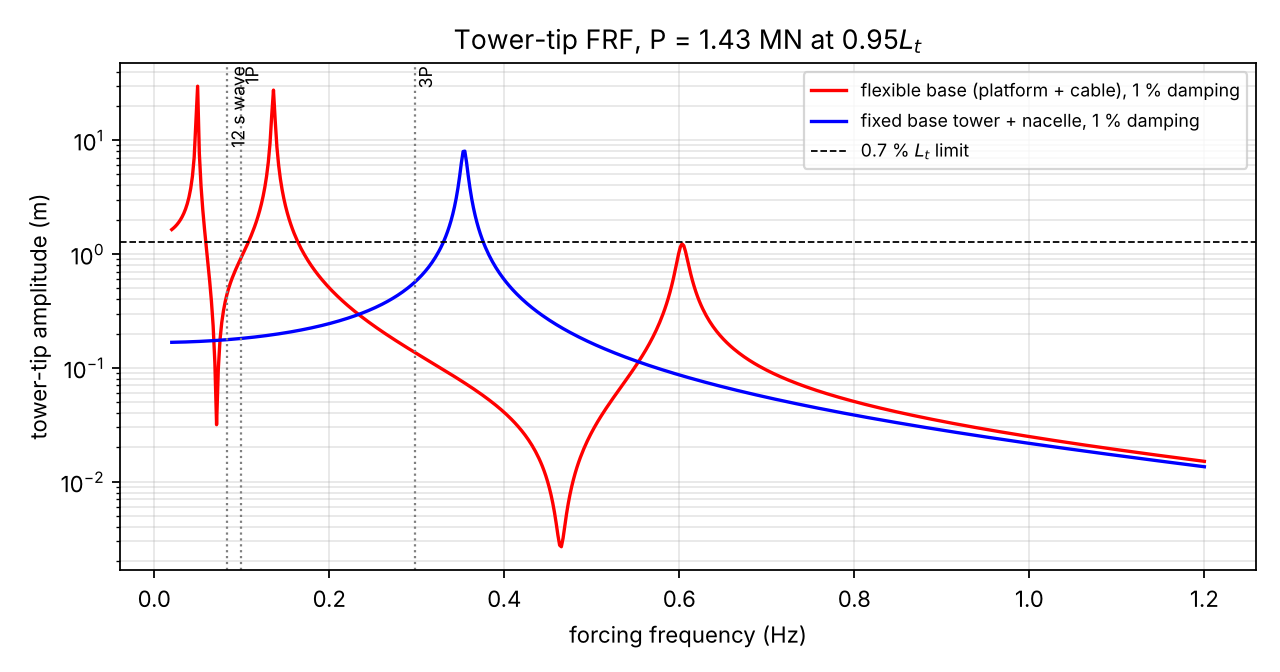
\includegraphics[width=0.9\textwidth]{fe_frf.png}
\caption{Tower-tip frequency response to $P=1.43\,\mathrm{MN}$ at $0.95L_t$ with $1\%$ modal damping. The flexible base moves the first peak from $0.354$ to $0.136\,\mathrm{Hz}$ and places 1P on its flank; the anti-resonance at $0.071\,\mathrm{Hz}$, between the surge mode ($0.049\,\mathrm{Hz}$) and the coupled mode, is where the platform surge motion acts as a vibration absorber for the tower tip.}
\label{fig:frf}
\end{figure}

\subsection*{Sensitivity of the coupled mode (FE runs)}
\begin{table}[H]
\centering
\caption{Coupled pitch--bending mode from the flexible-base FE model under single-parameter changes (all other inputs as in Table~\ref{tab:fe}).}
\label{tab:sens}
\begin{tabular}{@{}lcc@{}}
\toprule
Run & Coupled mode (Hz) & Surge (Hz) \\
\midrule
Baseline (Timoshenko, $T_{pc}=400$ kN, $b=40$ m, $k_x=0.5$ MN/m) & 0.1361 & 0.0490 \\
Euler--Bernoulli elements (no shear, no rotary inertia) & 0.1363 & 0.0490 \\
Tower $EI$ doubled & 0.1386 & 0.0491 \\
Column spacing $b=50$ m ($4k_yb^2$ up 56\%) & 0.1661 & 0.0491 \\
Mooring stiffness $k_x\to0.314k_x$ (A2.3 reduction) & 0.1356 & 0.0276 \\
Cable tension removed & 0.1361 & 0.0490 \\
\bottomrule
\end{tabular}
\end{table}
\subsection*{Recommended vibration control}
\begin{enumerate}
\item \textbf{Do not stiffen the tower further.} $f_1$ of the coupled mode is set by the platform pitch stiffness $4k_yb^2$ and the tower/nacelle inertia, not by $EI$: doubling $EI$ moves it from $0.136$ to only $0.139\,\mathrm{Hz}$ (Table~\ref{tab:sens}).
\item \textbf{Platform pitch stiffness.} The mode scales with $b$: widening the column spacing from $40$ to $50\,\mathrm{m}$ raises $4k_yb^2$ by $56\%$ and the coupled mode to $0.166\,\mathrm{Hz}$ (Table~\ref{tab:sens}), moving the 3P crossing to $U_\infty\approx8.4\,\mathrm{m/s}$; it does not remove it.
\item \textbf{Nacelle tuned mass damper} (the control that addresses the amplitude directly). The effective modal mass of the $0.136\,\mathrm{Hz}$ mode referred to the tower tip is $m_{eff}=\boldsymbol\phi^T\mathbf M\boldsymbol\phi/\phi_{tip}^2=636\,\mathrm{t}$. Applying the A2.5 rule (both split frequencies at least $35\%$ from the uncontrolled mode, lower branch governing, $\mu=0.789$):
\[
m_a=0.789\times636=\mathbf{502\,\mathrm{t}},\qquad k_a=m_a(2\pi\times0.136)^2=\mathbf{367\,\mathrm{kN/m}},
\]
tuned to the coupled frequency from this FE model, not to the fixed-base $0.357\,\mathrm{Hz}$ -- an absorber tuned to the B2.1 value would be $2.6\times$ off and ineffective. With realistic absorber damping ($\zeta_a\approx0.1$) the same device also provides the doubled modal damping recommended in B1.4 and A1.4.
\item \textbf{Operational.} A rotor-speed exclusion band around $\Omega_b=0.285\,\mathrm{rad/s}$ ($U_\infty\approx6$--$8\,\mathrm{m/s}$) removes the 3P crossing of the coupled mode at negligible energy cost, and should be combined with item~3.
\end{enumerate}

\section*{Code and data availability}\label{sec:code}
\addcontentsline{toc}{section}{Code and data availability}
{\small All scripts, results and geometry for this report are in the public repository
\begin{center}
\url{https://github.com/GITHUB-USERNAME/mech3200-b2-fowt}
\end{center}
\begin{itemize}[nosep]
\item \texttt{fe\_model.py} -- the planar finite-element model of Section~\ref{sec:b24} (Timoshenko beam elements, geometric stiffness for the tensioned cable, rigid-platform master--slave constraints, modal and forced solutions). Running it reproduces Tables~\ref{tab:validation}, \ref{tab:fe} and \ref{tab:sens}, Figures~\ref{fig:modes}--\ref{fig:frf}, and writes \texttt{fe\_results.json}.
\item \texttt{analytical.py} -- the B2.1--B2.3 design calculations (cantilever and tip-mass characteristic equations, modal forced response, diameter and thickness sizing); writes \texttt{analytical.json}.
\item \texttt{make\_step.py} -- generates the STEP geometry \texttt{MECH3200\_B2\_46555991.step} and \texttt{B2\_tower\_only.step} from the design values.
\item \texttt{fe\_results.json}, \texttt{analytical.json} -- the numerical output quoted in the text; the PNG figures; the \LaTeX{} source. The commit tagged \texttt{submission} is the version used for every number here (Python~3, NumPy, SciPy, Matplotlib; CadQuery for STEP export only).
\end{itemize}}
\end{document}
